\documentclass[aspectratio=169,dvipdfmx,14pt,notheorems]{beamer}
%%%% 和文用 %%%%%
\usepackage{bxdpx-beamer}
\usepackage{pxjahyper}
\usepackage{minijs}%和文用
\renewcommand{\kanjifamilydefault}{\gtdefault}%和文用

%%%% スライドの見た目 %%%%%
\usetheme{Madrid}
\usefonttheme{professionalfonts}
\setbeamertemplate{frametitle}[default][center]
\setbeamertemplate{navigation symbols}{}
\setbeamercovered{transparent}%好みに応じてどうぞ)
\setbeamertemplate{blocks}[rounded]
\useinnertheme{circles}
\setbeamertemplate{footline}[page number]
\setbeamerfont{footline}{size=\normalsize,series=\bfseries}
\setbeamercolor{footline}{fg=black,bg=black}
%%%%

%%%% 定義環境 %%%%%
\usepackage{amsmath,amssymb}
\usepackage{amsthm}
\theoremstyle{definition}
\newtheorem{theorem}{定理}
\newtheorem{definition}{定義}
\newtheorem{proposition}{命題}
\newtheorem{lemma}{補題}
\newtheorem{corollary}{系}
\newtheorem{conjecture}{予想}
\newtheorem*{remark}{Remark}
\renewcommand{\proofname}{}
%%%%%%%%%

%%%%% フォント基本設定 %%%%%
\usepackage[T1]{fontenc}%8bit フォント
\usepackage{textcomp}%欧文フォントの追加
\usepackage[utf8]{inputenc}%文字コードをUTF-8
\usepackage[deluxe]{otf}%otfパッケージ
\usepackage{lxfonts}%数式・英文ローマン体を Lxfont にする
\usepackage{bm}%数式太字
%%%%%%%%%%

%%%%% PythonTeX %%%%%
\usepackage[makestderr]{pythontex}
\restartpythontexsession{\thesection}
 
\title{組み込み関数powの知られざる進化}
\subtitle{Unknown Evolution of the Built-in Function pow}
\author[Hayao]{Hayao Suzuki}
\institute[PyCon JP 2021]{PyCon JP 2021}
\date{October 15, 2021}

\begin{document}

\begin{frame}[plain]\frametitle{}
\titlepage %表紙
\end{frame}

\begin{frame}\frametitle{発表に際して}

\begin{block}{GitHubに資料があります}
\begin{itemize}
\item \url{https://github.com/HayaoSuzuki/pyconjp2021}
\end{itemize}
\end{block}

\begin{block}{Twitterのハッシュタグ}
\begin{itemize}
\item \#pyconjp \#pyconjp\_3
\end{itemize}
\end{block}

\begin{block}{PyCon JP Discord}
\begin{itemize}
\item \#jp-2021-track-3 TBA
\end{itemize}
\end{block}
\end{frame}

\section{はじめに}

\begin{frame}\frametitle{Who am I ?}

\begin{block}{お前誰よ}
\begin{description}
\item[名前] Hayao Suzuki(鈴木 駿)
\item[Twitter] \href{https://twitter.com/CardinalXaro}{@CardinalXaro}
\item[仕事] Software Developer @ BeProud Inc.
\end{description}
\end{block}

%\begin{center}
%\begin{itemize}
%\item 株式会社ビープラウド \includegraphics[width=4cm]{bplogo.png}
%\begin{itemize}
%\item IT勉強会支援サービス connpass \includegraphics[width=2cm]{connpass_logo_1.png}
%\item オンライン学習サービス PyQ \includegraphics[width=1cm]{pyq_logo_color.png}
%\item システム開発のためのドキュメントサービス Tracery
%\end{itemize}
%\end{itemize}
%\end{center}

\end{frame}

\begin{frame}\frametitle{Who am I ?}

\begin{block}{監訳・査読した技術書(抜粋)}
\begin{itemize}
\item \structure{入門 Python 3 第2版}(O'Reilly Japan)
\item \structure{Effective Python 第2版}(O'Reilly Japan)
\item \structure{機械学習による実用アプリケーション構築}(O'Reilly Japan)
\item \structure{PyTorchとfastaiではじめるディープラーニング}(O'Reilly Japan)
\item \structure{実践 時系列解析}(O'Reilly Japan) \structure{New!}
\item \structure{機械学習デザインパターン}(O'Reilly Japan) \structure{New!}
\end{itemize}
\end{block}
\url{https://xaro.hatenablog.jp/}にリストがあります。
\end{frame}

\begin{frame}\frametitle{Who am I ?}

\begin{block}{発表リスト(抜粋)}
\begin{itemize}
\item \structure{レガシーDjangoアプリケーションの現代化}(DjangoCongress JP 2018)
\item \structure{SymPyによる数式処理}(PyCon JP 2018)
\item \structure{Pythonと楽しむ初等整数論}(PyCon mini Hiroshima 2019)
\item \structure{君はcmathを知っているか}(PyCon mini Shizuoka 2020)
\item \structure{インメモリーストリーム活用術}(PyCon JP 2020)
\end{itemize}
\end{block}
\url{https://xaro.hatenablog.jp/}にリストがあります。
\end{frame}

\begin{frame}\frametitle{今日の目標}

\begin{block}{組み込み関数\texttt{pow}}
\begin{itemize}
\item \texttt{pow}関数は数のべき乗を返す関数
\item Pythonに限らず、大抵の言語には\texttt{pow}関数が存在する
\end{itemize}
\end{block}

\begin{exampleblock}{Python 3.8で機能追加}
\begin{itemize}
\item 整数$m$を法とする剰余類における乗法逆元が計算できる
\item よくわからない単語を並べるな!
\end{itemize}
\end{exampleblock}
\end{frame}

\begin{frame}\frametitle{今日の目標}
\begin{block}{組み込み関数\texttt{pow}の知られざる進化}
\begin{itemize}
\item Python 3.8で追加された\texttt{pow}関数の新機能を理解する
\item 「整数$m$を法とする剰余類における逆元」の意味を理解する
\item 「整数$m$を法とする剰余類における逆元」を計算するアルゴリズムを理解する
\end{itemize}
\end{block}
\end{frame}

\section{従来のpow関数}

\begin{frame}\frametitle{今までの\texttt{pow}関数}
\begin{center}
\Large Python 3.7までの\texttt{pow}関数を復習しよう
\end{center}
\end{frame}

\subsection{数のべき乗について}

\begin{frame}\frametitle{整数のべき乗}
\begin{definition}[整数のべき乗]
整数$b$と自然数$n$に対して、\structure{べき乗}$b^{n}$を
\begin{equation*}
b^{n} \triangleq \overbrace{b \times b \times \cdots \times b}^{n\text{個}}
\end{equation*}
と定義する。$b$を\structure{底}、$n$を\structure{指数}と呼ぶ。
\end{definition}

\begin{exampleblock}{整数のべき乗の例}
\begin{equation*}
2^{32} = 4294967296.
\end{equation*}
\end{exampleblock}

\end{frame}

\begin{frame}[fragile]\frametitle{整数のべき乗}

\begin{block}{Pythonにおけるべき乗}
組み込み関数\texttt{pow}または\texttt{**}演算子を使う。
\end{block}

\begin{exampleblock}{べき乗の実行例}

\begin{pyconsole}
pow(2, 32)
2 ** 32
\end{pyconsole}

\end{exampleblock}
% メモ int型におけるpowの実装は以下の通り
% https://github.com/python/cpython/blob/59242431991794064824cf2ab70886367613f29e/Objects/longobject.c#L4097
% Left-to-right binary exponentiation と呼ばれるアルゴリズムを使っている

\end{frame}

\subsection{べき乗剰余について}

\begin{frame}\frametitle{べき乗剰余}
\begin{definition}[べき乗剰余]
自然数の底$b$と自然数$n, m$に対して、
\begin{equation*}
b^{n} \bmod{m}
\end{equation*}
を\structure{$m$を法とするべき乗剰余}と定義する。
\end{definition}

\begin{exampleblock}{べき乗剰余の例}
\begin{equation*}
2^{32} \bmod{65535} = 1.
\end{equation*}
\end{exampleblock}

\end{frame}

\begin{frame}[fragile]\frametitle{べき乗剰余}

\begin{block}{Pythonにおけるべき乗剰余}
\begin{itemize}
\item 組み込み関数\texttt{pow}で\structure{効率的に}計算できる。
\item \texttt{**}演算子および\texttt{\%}演算子でも計算可能だが\structure{効率が悪い}。
\item Python 1.5から利用可能。
\end{itemize}
\end{block}

\begin{exampleblock}{べき乗剰余の実行例}

\begin{pyconsole}
pow(2, 262144, 65535)
(2 ** 262144) % 65535
\end{pyconsole}

% メモ
% 計算の都度、余りを計算してるように見えるが、ちょっと自身がない
% https://github.com/python/cpython/blob/59242431991794064824cf2ab70886367613f29e/Objects/longobject.c#L4219

% めも
% 1.5の該当ドキュメント、但し int の範囲に収まる必要がある
% https://docs.python.org/release/1.5/lib/node26.html#1810

\end{exampleblock}

\end{frame}

\begin{frame}[fragile]\frametitle{べき乗剰余}

\begin{exampleblock}{どれだけ効率的か}

\begin{pyconsole}
import timeit
timeit.timeit("pow(2, 262144, 65535)", number=1000)
timeit.timeit("(2 ** 262144) % 65535", number=1000)
\end{pyconsole}

\end{exampleblock}
結果を実行回数で割れば平均時間がわかる。

\end{frame}

\begin{frame}[fragile]\frametitle{べき乗剰余}

\begin{exampleblock}{演算子と関数における計算時間の比較}
\begin{figure}
  \centering
  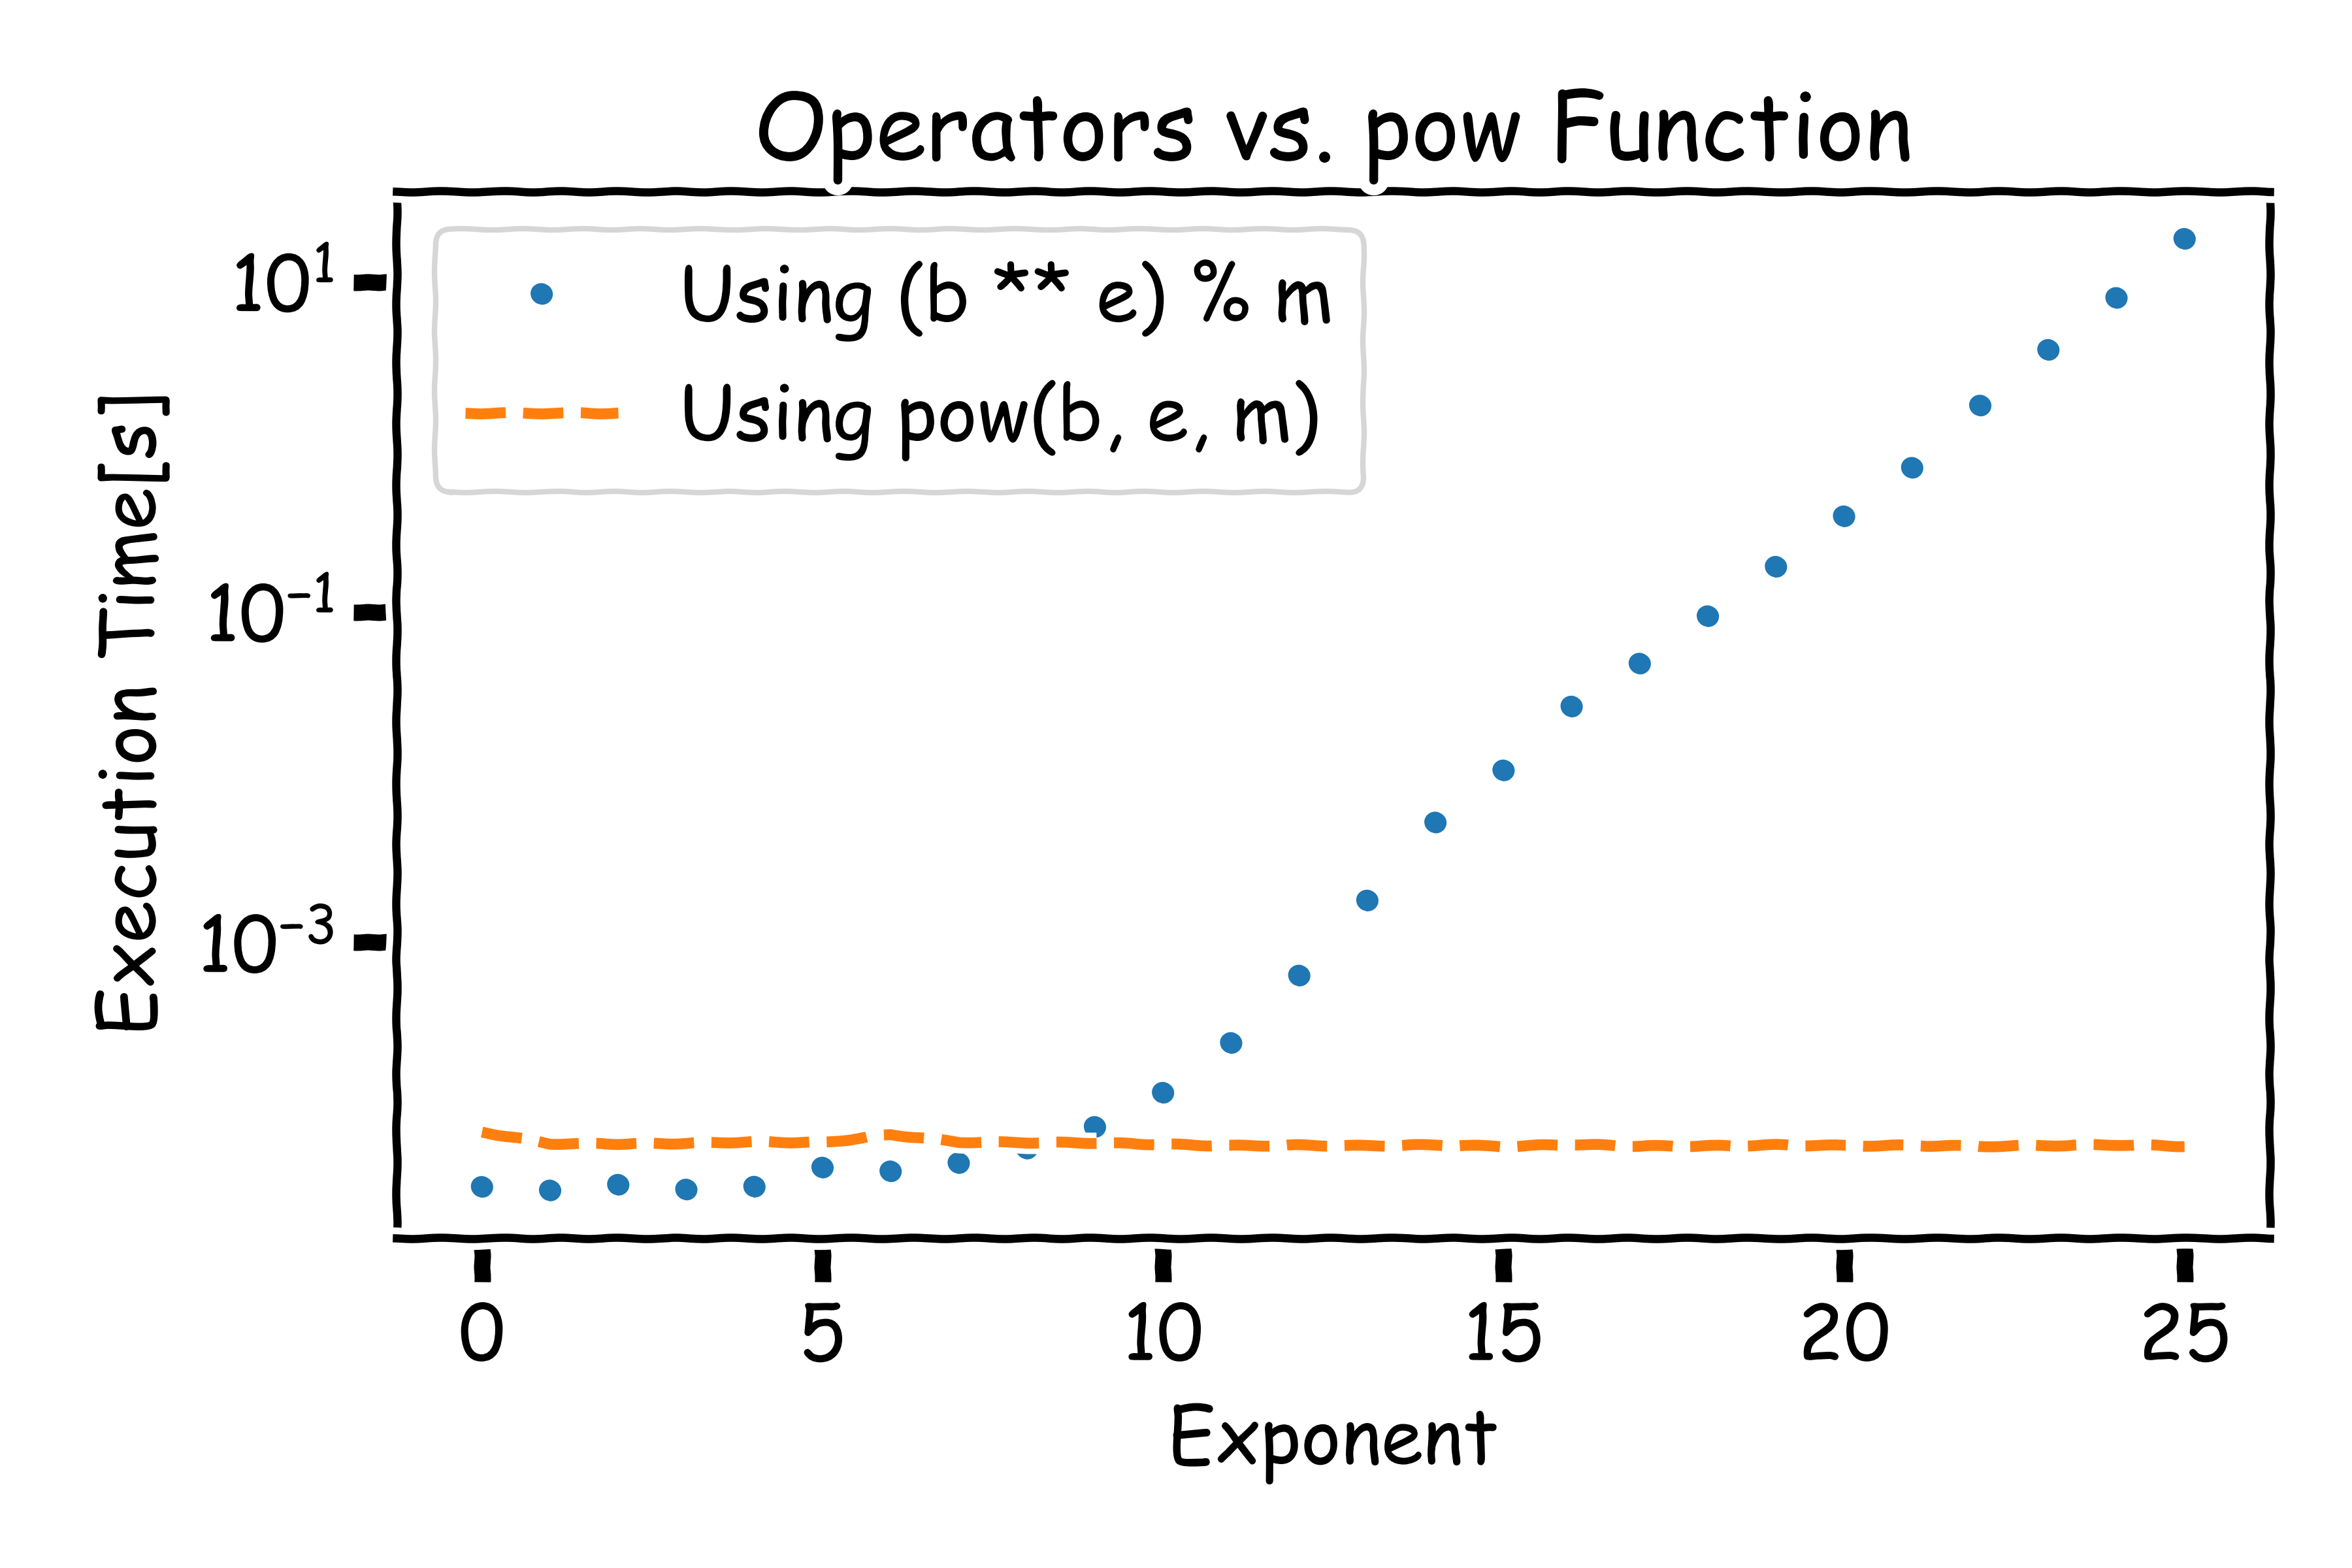
\includegraphics[width=9cm]{op_vs_func.png}
\end{figure}
\end{exampleblock}

\end{frame}


\section{Python 3.8からのpow関数}

\begin{frame}\frametitle{これからの\texttt{pow}関数}
\begin{center}
\Large Python 3.8からの\texttt{pow}関数を理解するために
\end{center}
\end{frame}

\subsection{整数の合同}

\begin{frame}\frametitle{整数の合同}

\begin{definition}[整数の合同]
整数$a$が$m$を法として$b$と合同であるとは$m$が$a-b$を割り切ることをいい、
\begin{equation*}
a \equiv b \pmod{m}
\end{equation*}
と表す。
\end{definition}

\begin{exampleblock}{整数の合同の例}
\begin{equation*}
47 \equiv 35 \pmod{6}
\end{equation*}
$47-35 = 12$は6で割り切れる。
\end{exampleblock}

\end{frame}

\subsection{乗法逆元の定義}

\begin{frame}\frametitle{これからの\texttt{pow}関数}

\begin{definition}[整数$m$を法とする剰余類における乗法逆元]
整数$a, b$と自然数$m$に対して、
\begin{equation*}
ab \equiv 1 \pmod{m}
\end{equation*}
となるとき、$b$を$a$の\structure{乗法逆元}と呼び、$a^{-1}$と表す。
\end{definition}

\begin{exampleblock}{剰余類における乗法逆元の例}
\begin{equation*}
38 * 23 \equiv 1 \pmod{97}
\end{equation*}
38の97を法とする乗法逆元は23
\end{exampleblock}

\end{frame}

\begin{frame}[fragile]\frametitle{剰余類における乗法逆元}

\begin{block}{Pythonにおける剰余類における乗法逆元}
\begin{itemize}
\item 組み込み関数\texttt{pow}の第2引数に$-1$を渡せば計算可能
\item これがPython 3.8の新機能
\end{itemize}
\end{block}

\begin{exampleblock}{剰余類における乗法逆元の実行例}

\begin{pyconsole}
pow(38, -1, 97)
(38 * 23) % 97 == 1
\end{pyconsole}

\end{exampleblock}

\end{frame}

\subsection{乗法逆元が存在する条件}

\begin{frame}[fragile]\frametitle{剰余類における乗法逆元}

\begin{alertblock}{必ずしも乗法逆元が存在するとは限らない}

\begin{pyconsole}
pow(2, -1, 6)
\end{pyconsole}
\end{alertblock}
与えられた法に対して底が乗法逆元を持たない(何故?)。
\end{frame}

\begin{frame}[fragile]\frametitle{乗法逆元を求めて}

\begin{block}{乗法逆元の意味}
整数$a$に対して、$m$を法とする合同方程式
\begin{equation*}
ax \equiv 1 \pmod{m}
\end{equation*}
を解くことに他ならない。
\end{block}

\end{frame}

\begin{frame}[fragile]\frametitle{合同の定義に立ち返る}

\begin{block}{乗法逆元の意味}
$ax \equiv 1 \pmod{m}$を変形すると、不定方程式
\begin{equation*}
ax -my = 1
\end{equation*}
が整数解$x, y$を持つことに他ならない。
\end{block}

\end{frame}

\begin{frame}[fragile]\frametitle{方程式を観察する}

\begin{exampleblock}{例:$3x + 9y$なる数式}
$x$や$y$に整数を代入するといずれも3の倍数となる。
\begin{table}[]
\begin{tabular}{|c|c|c|c|c|c|}
\hline
       & $x=-2$ & $x=-1$ & $x=0$ & $x=1$ & $x=2$ \\ \hline
$y=-2$ & -24    & -21    & -18   & -15   & -12   \\ \hline
$y=-1$ & -15    & -12    & -9    & -6    & -3    \\ \hline
$y=0$  & -6     & -3     & 0     & 3     & 6     \\ \hline
$y=1$  & 3      & 6      & 9     & 12    & 15    \\ \hline
$y=2$  & 12     & 15     & 18    & 21    & 24    \\ \hline
\end{tabular}
\end{table}

\end{exampleblock}

\end{frame}

\begin{frame}[fragile]\frametitle{合同方程式の解}

\begin{theorem}
整数$a, c$に対して、$m$を法とする合同方程式
\begin{equation*}
ax \equiv c \pmod{m}
\end{equation*}
は、$c$が$\gcd(a, m)$で割り切れるときのみ、ちょうど$\gcd(a, m)$個の互いに合同ではない解を持つ。
ただし、$\gcd(a, m)$は$a$と$m$の最大公約数である。
\end{theorem}
証明は、適当な初等整数論の教科書を参照してください。
\end{frame}

\begin{frame}[fragile]\frametitle{今回のケース}

\begin{corollary}
整数$a,$に対して、$m$を法とする合同方程式
\begin{equation*}
ax \equiv 1 \pmod{m}
\end{equation*}
は、$\gcd(a, m) = 1$の場合のみ、1個の互いに合同ではない解を持つ。
\end{corollary}
乗法逆元が存在するかどうかは数学的な裏付けがある。
\end{frame}

\begin{frame}[fragile]\frametitle{剰余類における乗法逆元}

\begin{exampleblock}{乗法逆元が存在するケース}

\begin{pyconsole}
import math
math.gcd(38, 97)
pow(38, -1, 97)
\end{pyconsole}
\end{exampleblock}
$\gcd(38, 97) = 1$なので、97を法とする38の乗法逆元が存在する。
\end{frame}


\begin{frame}[fragile]\frametitle{剰余類における乗法逆元}

\begin{alertblock}{乗法逆元が存在しないケース}

\begin{pyconsole}
import math
math.gcd(2, 6)
pow(2, -1, 6)
\end{pyconsole}
\end{alertblock}
$\gcd(2, 6) \neq 1$なので、6を法とする2の乗法逆元は存在しない。
\end{frame}

\subsection{拡張Euclidの互除法}

\begin{frame}[fragile]\frametitle{Euclidの互除法}
\begin{theorem}
$a, b$を$a \leq b$である整数、$r$を$a$を$b$で割った余りとする。
このとき、
\begin{equation*}
\gcd(a, b) = \gcd(b, r)
\end{equation*}
が成り立つ。
\end{theorem}
\end{frame}

\begin{frame}[fragile]\frametitle{Euclidの互除法}
\begin{block}{Euclidの互除法と1次不定方程式}
$a$を$b$で割った商と剰余をそれぞれ$q, r$とする。
不定方程式$ax+by=1$に$a = qb + r$を代入すると、
\begin{align*}
& (qb + r)x + by = 1 \\
\Rightarrow & b(qx + y) + rx = 1
\end{align*}
となる。
\end{block}
つまり、$ax+by=1$から$bs + rt = 1$にすることができる。

$x=t, y = s - qt$という関係。
\end{frame}

\begin{frame}[fragile]\frametitle{Euclidの互除法}
\begin{exampleblock}{97と38の最大公約数を計算する}
\begin{align*}
97 &= 2 \times 38 + 21 \\
38 &= 1 \times 21 + 17 \\
21 &= 1 \times 17 + 4 \\
17 &= 4 \times 4 + 1 \\
4 &= 1 \times 4 + 0
\end{align*}
\end{exampleblock}
\end{frame}

\begin{frame}[fragile]\frametitle{Euclidの互除法}
\begin{exampleblock}{97と38の最大公約数を計算する}
$a=97, b=38$とすると
\begin{align*}
21 &= a -2b \\
17 &= b -21 \\
     &= -a + 3b \\
4   &= 21 - 17 \\
     &= 2a - 5b \\
1 &= 17 - 4 \times 4 \\
   &= -9a + 23b
\end{align*}
\end{exampleblock}
\end{frame}

\begin{frame}[fragile]\frametitle{Euclidの互除法}
\begin{theorem}{不定方程式}
$a, b$を0ではない整数とする。このとき、方程式
\begin{equation*}
ax + by = \gcd(a, b)
\end{equation*}
は解$(x_{0}, y_{0})$を持ち、Euclidの互除法によって求めることができる。
\end{theorem}
\end{frame}

\begin{frame}[fragile]\frametitle{\texttt{pow}の中身}
\begin{block}{\texttt{longobject.c}のコメントにある実装(一部改変)}
\begin{pygments}{python}
def invmod(a, m):
    x, y = 1, 0
    while m:
        q, r = divmod(a, m)
        a, m = m, r
        x, y = y, x - q * y
    if a == 1:
        return x
    raise ValueError("Not invertible")
\end{pygments}
\end{block}
\end{frame}


\section{まとめ}

\begin{frame}[fragile]\frametitle{Conclusion}
\begin{block}{まとめ}
\begin{itemize}
\item \texttt{pow}関数は数のべき乗を返す関数である。
\item べき乗剰余を計算する場合は必ず\texttt{pow}関数を使う。
\item Python 3.8で剰余類の乗法逆元が計算できるようになった。
\item 乗法逆元が計算できる仕組みはEuclidの互除法にある。
\end{itemize}
\end{block}
\texttt{pow}関数とEuclidの互除法ゎ…ズッ友だょ…!!
\end{frame}
\end{document}
